\documentclass[12pt, a4paper]{article}


\usepackage[margin=0.9in]{geometry}
\usepackage{graphicx}
\usepackage{float}
\usepackage{hyperref}
\usepackage{xcolor}
\definecolor{cvgreen}{RGB}{95,187,67}
\usepackage{hyperref}
\hypersetup{
	colorlinks,
	citecolor=cvgreen,
	filecolor=black,
	linkcolor=black,
	urlcolor=blue
}

\usepackage{listings}
\lstset{
	basicstyle=\ttfamily,
	columns=fullflexible,
	language=C,
	numbers=none,
	stepnumber=1,
	frame=none,
	breaklines=true,
	showstringspaces=false,
	postbreak=\mbox{\textcolor{red}{$\hookrightarrow$}\space},
	basicstyle=\footnotesize\ttfamily,
	keywordstyle=\bfseries\color{green},
	commentstyle=\itshape\color{red},
	identifierstyle=\color{blue},
	stringstyle=\color{black},
}


\title{\Huge{Bias in Word Embeddings}\\ \vspace{2mm} \Large{Project Report}}
\author{Ankit Pant -- 2018201035 \\ Tarun Mohandas -- 2018201008 \\
	Supervised by: Dr. Manish Shrivastava}
\date{}

\begin{document}
	\maketitle
	\thispagestyle{empty}
	\noindent\rule{\textwidth}{1pt}
	\newpage
	\pagenumbering{roman}
	\setcounter{page}{1}
	\begin{abstract}
		Word embeddings are a type of word representation that allows words with similar meaning to have a similar representation. The blind application of machine learning on Web embeddings runs the risk of amplifying biases present in data. Word embeddings trained on a standard Natural Language Processing datasets, exhibit female/male gender stereotypes to a disturbing extent. Not only that a lot of other biases like racial bias and religious bias is also present. This raises concerns because their widespread use, often tends to amplify these biases.
		\par The project aims to explore bias present in word embeddings and the techniques used to reduce/eliminate this. 	\end{abstract}
	\newpage
	
	\tableofcontents
	\newpage
	
	\pagenumbering{arabic}
	\setcounter{page}{1}
	
	\section{Introduction}
		Word embeddings are one the most popular representations of words that are used in Natural Language Processing (NLP) tasks. However it has been determined that these inherently contain various types of biases \cite{5,6}, with gender bias, racial bias, and religious bias among them. The problem of the word embeddings containing these biases is further aggravated by their use in various tasks in NLP. The reliance on Machine Learning (ML) and Artificial Intelligence (AI) is ever increasing and various ML and AI techniques are being employed in a variety of tasks -- from resume shortlisting to identifying potential criminals \cite{7}. 
		\par Hence it becomes increasingly important that biases in the word embeddings are eliminated so that the algorithms do not inadvertently amplify these biases and result in a disadvantage to a particular social group.
		\par This project looks at some of these biases and attempts to use existing debiasing technique to see their effect. We also look at some shortcomings of this debiasing technique  \cite{1} and seek some improvements. 
	\section{Literature Review}
		
		\subsection{Word Embeddings}
			Word embedding is one of the most popular representation of document vocabulary. It is capable of capturing context of a word in a document, semantic and syntactic similarity, relation with other words, etc. They are vector representations of a particular word. \emph{Word2Vec} is one of the most popular technique to learn word embeddings using shallow neural network. 
			\par
			\emph{Word2Vec} can utilize either of two model architectures to produce a distributed representation of words: continuous bag-of-words (CBOW) or continuous skip-gram. In the continuous bag-of-words architecture, the model predicts the current word from a window of surrounding context words. The order of context words does not influence prediction. In the continuous skip-gram architecture, the model uses the current word to predict the surrounding window of context words. The skip-gram architecture weighs nearby context words more heavily than more distant context words.
			
		\subsection{Types of Bias}
			It is important to quantify and understand bias in languages as such biases can reinforce the psychological status of different groups \cite{4}. Biases differ across people though commonalities can be detected. A number of online systems have been shown to exhibit various biases, such as racial discrimination and gender bias in the ads presented to users. Different demographic and geographic groups also use different dialects and word-choices in social media. An implication of this effect is that language used by minority group might not be able to be processed by natural language tools that are trained on ``standard” data-sets. The following subsections elaborate on the different kinds of bias that can be in word embeddings.
			
			\subsubsection{Historical Bias}
				It captures the unwanted biases that were present in society years ago. Since word embeddings are trained on various literature, historical literature containing these biases inadvertently make into the word embeddings.
				
			\subsubsection{Representational Bias} 
				This occurs when certain parts of the input space are under-represented. It occurs when the input distribution contains very few examples of a particular part of the input \cite{8}.
				
			\subsubsection{Measurement Bias}
				This occurs as a consequence of imperfect measuring of the data, that is, assuming that the measured data is a proxy of some other desired feature \cite{8}. Often instead of random noise, each kind of proxy has its own kind of noise giving rise to measurement bias.
				
			\subsubsection{Aggregation Bias}
				This kind of bias arises when the same model is used for groups with different conditional distributions \cite{8}. Aggregation bias cause a model to be unfit for any of those distributions.
				
			\subsubsection{Evaluation Bias}
				This occurs when the evaluation and benchmark data for the model does not represent the actual target population \cite{8}. It often arises due to the need to objectively compare different models.
			
		\subsection {Social Biases in Datasets}
		
			\subsubsection{Gender Bias}
				Gender bias in language has been studied over a number of decades in a variety of contexts. Common biases link female terms with liberal arts and family and male terms with science and careers \cite{3}. While there are more words referring to males, there are many more words that discriminates females than males. The following are some of common gender biases found in the standard datasets:
				\begin{enumerate}
					\item Man is to computer programmer as woman is to homemaker
					\item Man is to doctor as woman is to nurse
				\end{enumerate}
				
				Although the aforementioned examples prominently show gender bias, the following associations does not show any malignant bias and need not be modified.
				
				\begin{enumerate}
					\item Man is to king as woman is to queen
					\item Man is to actor as woman is to actress
				\end{enumerate}
				
				Since the aforementioned examples have gender specific modifications to the words, they do not show unhealthy bias towards any gender.
				
			
			\subsubsection{Racial Bias}
				Racial Bias poses a problems to the systems that need to take decisions on people belonging to various communities and races. A grave example of such a system is COMPAS which is used to forecast which criminals will re-offend \cite{9}. This system has been shown to be biased against (Black) African-Americans when compared to their (White) American counterparts. Racial Bias was also shown when in a study, job applications were sent in response to advertisements varying only name of candidates. It was found that European-American names (candidates) were 50\% more likely to be offered an interview opportunity \cite{10}.
				
			\subsubsection{Religious Bias}
				Religious Bias occurs with association of certain adjectives or phrases towards a particular religious community. This can pose similar (or even greater) threats as racial biases. The word embeddings associates certain words like terrorism to particular religion, while also associates different insults to other religions as well \cite{6}
		
		\subsection{Debiasing Techniques}
			Various debiasing techniques have been proposed that are currently used to debias word-embeddings. They involve both pre-processing of biased input as well as post-processing of trained word embeddings. The following subsections elaborate these techniques,
			
			\subsubsection{Hard debiasing}
				This is a post-processing technique of removing bias from trained word embeddings and was proposed by (Bolukbasi et al.) \cite{2}. It involves reducing the bias of those words that are not inherently gendered (e.g. father, mother, etc.). The gender projection is calculated and the projection of each word is made zero in the predefined gender direction ($ \vec{he} - \vec{she}$ or $ \vec{man} - \vec{woman}$).
				Mathematically it is represented as:
				\[ 
					\vec{w}_{biased} = \vec{w}\cdot(\vec{he} - \vec{she}) 
				\]
				\[				
					\vec{w}_{debiased} = \frac{(\vec{w} - \vec{w}_{biased})}{||{(\vec{w} - \vec{w}_{biased})||}}
				 \]
				 Hard debiasing involves two steps:
				 \begin{itemize}
				 	\item \textbf{Neutralize and Equalize:} This is also called Hard de-biasing. \emph{Neutralize} ensures that no gender-neutral words are present in the gender subspace and \emph{Equalize} equalises the set of words outside the subspace \cite{2}.
				 \end{itemize}
			 
			 \subsubsection{Soft debiasing}
			 	This is also a post-processing technique and was proposed by (Bolukbasi et al.) as well \cite{2}. According to the authors, [it] ``is a linear transformation that seeks to preserve pairwise inner products between all the word vectors while minimizing the projection of the gender neutral words onto the gender subspace" \cite{2}. Mathematically it is represented as:
			 	\[
			 		min_T \, {||{(TW)^T(TW) - W^TW}^2_F||} + \lambda {||{(TN)^T(TB)}^2_F||}
			 	\]
			 	
		 	\subsubsection{Learning General Neutral Word Embeddings}
		 		This is a pre-processing technique proposed by (Zhao et al.) \cite{3}. In this technique, the loss of the GloVe word embedding model is changed such that the gender information of the words gets concentrated to the last coordinate of each vector. Then these word representations are used without considering this last coordinate.
		
	\section{Methodology}
		The project first involved identifying the bias in the word embeddings used and then project them graphically to check their clustering. Then the hard debiasing technique is applied and the result are compared quantitatively as well as graphically. 
		
		\subsection{Dataset and Word Embeddings}
			Pre-trained word embeddings were used in this project. The word embeddings were sourced from the work of Thomas Manzini, et al. \cite{7,11}. The word embeddings were trained on the Reddit-L2 corpus \cite{12}. This dataset and the corresponding word embeddings were chosen as they reflect the vocabularies of common people. However one drawback of the dataset is that it involves American users at a higher proportion.
		
	\section{Experimentation and Results}
		The experimentation was done in multiple phrases and the corresponding details of the experiments and their corresponding results are elaborated in the following sub-sections.
		
		\subsection{Identifying Bias}
			The word embeddings were experimented with thorough various metrics like cosine distance, analogies, etc. to find the existence of various biases including gender bias, racial bias and religious bias. Some of the more interesting results obtained were:
			
			\subsubsection{Gender Bias}
				\begin{verbatim}
					Distance been man and homemaker: 	0.8588528782129288
					Distance been woman and homemaker: 0.5408898890018463
				\end{verbatim}
				Here we can clearly see that  the distance between man and woman for the same word is significant making the word associated with women.
				
				\begin{verbatim}
				manager is to man as mastercard is to woman
				programmer is to man as nutritionist is to woman
				secretary is to woman as chairman is to man
				teacher is to woman as professor is to man
				\end{verbatim}
				Here again the bias is obvious in the analogy task where corresponding to each profession, there is an association of professions highly associated with gender.
				
			\subsubsection{Racial Bias}
			\begin{verbatim}
			housewife is to white as drunkard is to black
			modern is to white as medieval is to black
			secretary is to black as chairman is to white
			filthy is to black as elitists is to white
			\end{verbatim}
			Here we can see bias between the white Americans and the Black Americans.
			
			\begin{verbatim}
			rich is to Indian as greedy is to American
			smart is to Indian as dishonest is to American
			manager is to American as barber is to Indian
			modern is to American as medieval is to Indian
			\end{verbatim}
			Here we see bias between Indians and Americans in the dataset.
			
			\subsubsection{Religious Bias}
				\begin{verbatim}
				manager is to Christian as dealer is to Muslim
				programmer is to Christian as lyft is to Muslim
				rich is to Christian as homeless is to Muslim
				housewife is to Christian as hooker is to Jew
				smart is to Christian as cheapskate is to Jew
				housewife is to Christian as crackhead is to Jew
				\end{verbatim}
			Here we see a bias between Christians, and Muslim and Jews. 
			\vspace{5mm}
			\par When we analysed the most biased words corresponding to the different subspaces the following results were obtained:
			
			\subsubsection{Most biased words in gender}
				For the gender subspace ($ \vec{man} - \vec{woman}$), \emph{magician} followed by \emph{carpenter} was the most male-dominated profession, and \emph{swear} followed by \emph{filthy} was the most male-dominated pronoun/word.
				
			\subsubsection{Most biased words in race}
				For the race subspace ($ \vec{indian} - \vec{american}$), \emph{butcher} followed by \emph{barber} was the most Indian-dominated profession, and \emph{lovely} followed by \emph{backpack} was the most Indian-dominated pronoun/word.
				
			\subsubsection{Most biased words in religion}
				For the race subspace ($ \vec{muslim} - \vec{christian}$), \emph{vet} followed by \emph{cop} was the most Muslim-dominated profession, and \emph{terrorist} followed by \emph{car} was the most Muslim-dominated pronoun/word.
				
			\subsection{Clustering of biased words}
				The inherent bias in the word embeddings cause a clustering effect where words having similar kinds of biases are grouped together. The following figures (\ref{profession-cluster-fig} and \ref{common-cluster-fig}) graphically depict this.
				
				\subsubsection{Clustering on Profession}
				\begin{figure}[H]
					\centerline{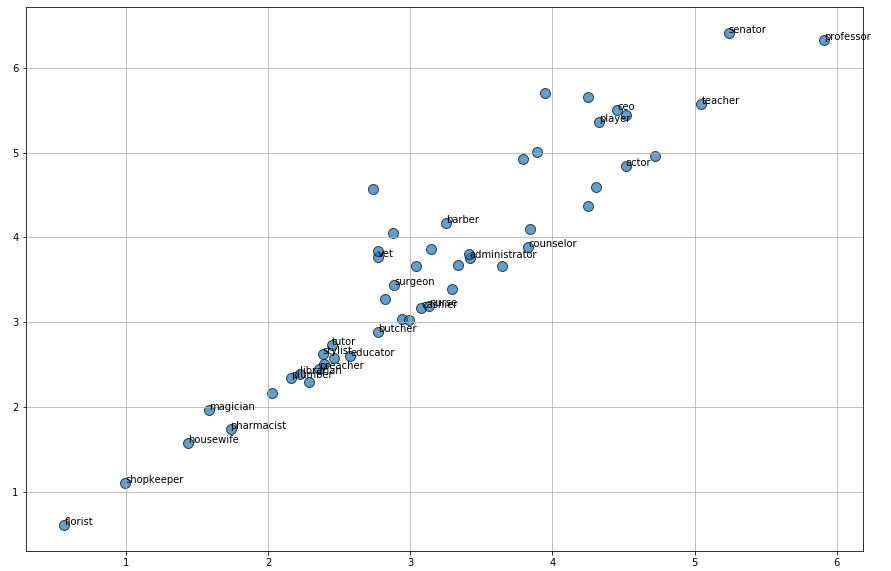
\includegraphics[width=25em]{biased_profession.png}}
					\caption{Result of clustering on male and female biased words}
					\label{profession-cluster-fig}
				\end{figure}
			
					\subsubsection{Clustering on Common Words}
				\begin{figure}[H]
					\centerline{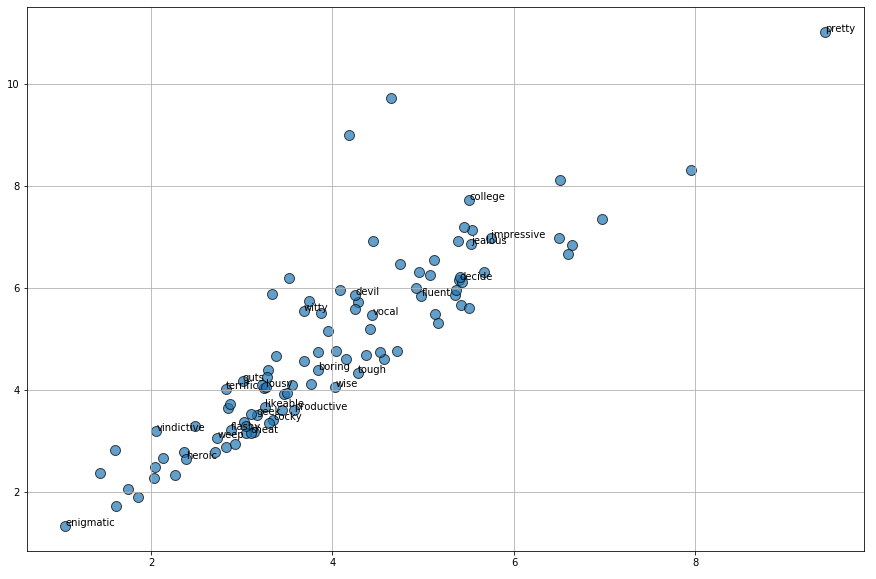
\includegraphics[width=25em]{biased_misc.png}}
					\caption{Result of clustering on male and female biased words}
					\label{common-cluster-fig}
				\end{figure}
			
			\subsection{Debiasing the word embeddings}
				To debias the word embeddings the hard-debiasing method was used \cite{2}. Debiasing was done on all three vector sub-spaces namely the gender sub-space, the race sub-space and the religion sub-space. The following result was obtained after applying the \emph{Neutralize} aspect of the hard debiasing technique.
				
				\subsubsection{For professions}
					\begin{verbatim}
						Bias in Professions in Model - decending order (top 10)
						
						('magician', 0.11574504) ==> ('magician', 0.11456225)
						('carpenter', 0.046477906) ==> ('carpenter', 0.045484226)
						('butcher', 0.035740644) ==> ('butcher', 0.035707153)
						('gamer', 0.027397364) ==> ('gamer', 0.026887717)
						('soldier', 0.018920997) ==> ('soldier', 0.019234942)
						('servant', 0.009307076) ==> ('servant', 0.008474963)
						('barber', 0.0073357197) ==> ('barber', 0.006497547)
						('engineer', -0.0022402948) ==> ('engineer', -0.0024358318)
						('player', -0.014475175) ==> ('player', -0.014581879)
						('programmer', -0.01649278) ==> ('programmer', -0.017327033)
					\end{verbatim}
				
				\subsubsection{For Common Words}
					\begin{verbatim}
						Bias in Misc. words in Model - descending order (top 10)
						
						('swear', 0.21706519) ==> ('swear', 0.21250035)
						('filthy', 0.20151068) ==> ('filthy', 0.19604209)
						('sweet', 0.19195326) ==> ('sweet', 0.18784045)
						('roar', 0.18197575) ==> ('roar', 0.17574164)
						('weep', 0.18006237) ==> ('weep', 0.17289506)
						('pretty', 0.17052722) ==> ('pretty', 0.16845691)
						('beautiful', 0.15033276) ==> ('beautiful', 0.14696142)
						('think', 0.1481186) ==> ('think', 0.14597465)
						('brave', 0.14424863) ==> ('brave', 0.14036529)
						('savage', 0.14332578) ==> ('savage', 0.13797511)
					\end{verbatim}
					
		\subsection{Clustering after debiasing}
			As per Hila et al. \cite{1}, even after applying traditional debiasing algorithm, the inherent bias still remains and these algorithms only remove the bias on a superficial level. We expected our results to also corroborate this argument hence plotted the clustering after debiasing as well. As expected the clustering pattern remained more or less the same even after the debiasing method was applied. The following figures (\ref{profession-debias-fig} and \ref{common-debias-fig}) graphically depict this.
			
				\subsubsection{Clustering on Profession}
				\begin{figure}[H]
					\centerline{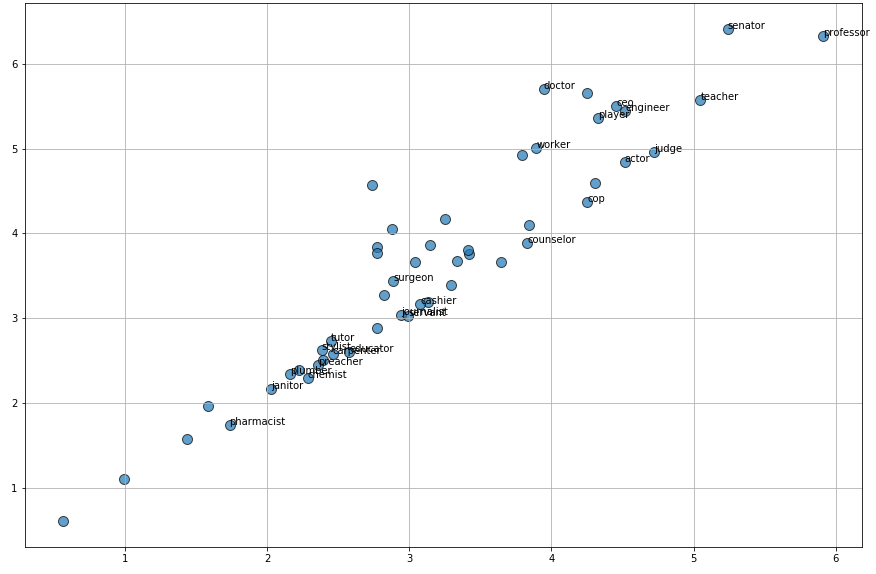
\includegraphics[width=25em]{debiased_profession.png}}
					\caption{Result of clustering on male and female biased words}
					\label{profession-debias-fig}
				\end{figure}
				
				\subsubsection{Clustering on Common Words}
				\begin{figure}[H]
					\centerline{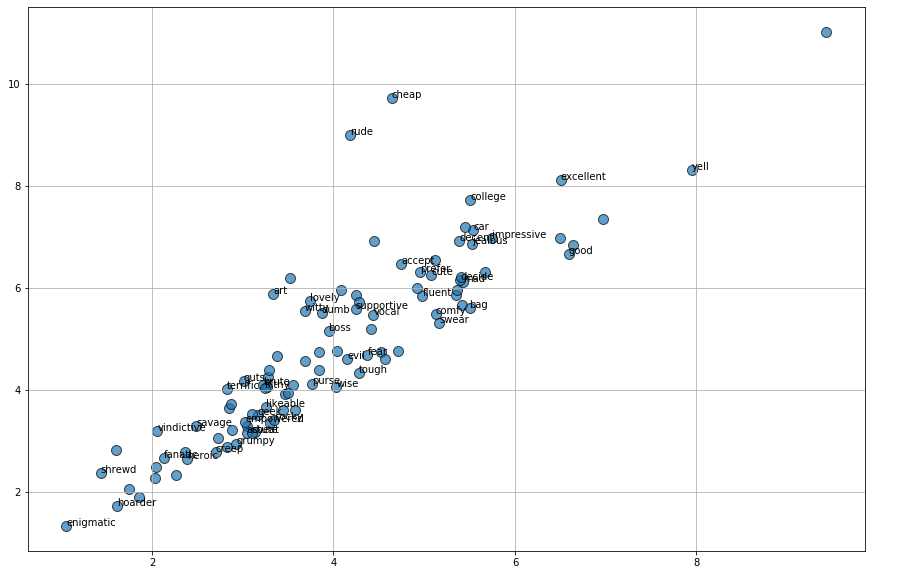
\includegraphics[width=25em]{debiased_misc.png}}
					\caption{Result of clustering on male and female biased words}
					\label{common-debias-fig}
				\end{figure}
			
	\section{Proposed Algorithm}
		After applying the traditional debiasing algorithm and still getting relative clustering of biased words we propose that an efficient an true debiasing algorithm must have the following components:
		\begin{itemize}
			\item Pre-processing the dataset so as to add sentences by inverting the gender, races, religion, etc. of the original sentences in the dataset and appending them to create a new dataset.
			\item Debiasing during pre-processing as with (Zhao et al.) \cite{3} would be beneficial to get the initial somewhat debiased word embeddings.
			\item  The words then must be analysed that propose the biases through the means of projecting them to the biased sub-space and debiased as done initially by (Bolukbasi et al.) \cite{2}.
			\item After identifying these words, they must be correlated with each other and the distances between the words clustering together should also be equalised.
		\end{itemize}
		On doing this equalisation we may ensure that words that were traditionally associated with a particular stereotype no longer clusters together with other such traditionally stereotypical words. This can possibly remedy the concerns put up by Hila et al. \cite{1} and enable a debiasing that is more concrete. However more understanding of how the word embeddings encode information would help to eliminate the bias.
		
			
	\section{Conclusion}
		The project involved exploring the different kinds of biases that are encoded into word embeddings and try and debias the embeddings. The word embeddings trained on the Reddit dataset were explored. An attempt to debias them using the traditional hard-debiasing method was also made. However as observed by Hila et al. \cite{1}, the debising happened on a superficial level. Another approach was hence proposed that would attempt to address this issue.
		
	\section{Future Scope}
		The project could be extended to further work on the proposed algorithm and implement it to empirically test if it indeed gives better results. The embedding process of the context of a word could also be explored to better understand how biases are encoded to remove them.
		
		
	\begin{thebibliography}{10}
		
		\bibitem{1} Hila Gonen, Yoav Goldberg, \textit{Lipstick on a Pig: Debiasing methods cover up systematic gender biases in word embeddings but do not remove them}, \url{https://arxiv.org/pdf/1903.03862.pdf}
		\bibitem{2} Tolga Bolukbasi, et al., \textit{Man is to Computer Programmer as Woman is to Homemaker? Debiasing Word Embeddings}, \url{https://arxiv.org/pdf/1607.06520.pdf}
		\bibitem{3} Jieyu Zhao, et al., \textit{Learning Gender-Neutral Word Embeddings}, \url{https://arxiv.org/pdf/1809.01496.pdf}
		\bibitem{4} Sevtap Duman, et al., \textit{(Visualization of) gender bias in word embeddings}, \url{http://wordbias.umiacs.umd.edu/}
		\bibitem{5}Aylin Caliskan, et al., \textit{Semantics derived automatically from language corpora contain human-like biases}, \url{https://arxiv.org/pdf/1608.07187.pdf}
		\bibitem{6}Nikhil Garg, et al., \textit{Word embeddings quantify 100 years of gender and ethnic stereotypes}, \url{https://arxiv.org/pdf/1711.08412.pdf}
		\bibitem{7} Thomas Manzini, et al., \textit{Black is to Criminal as Caucasian is to Police:Detecting and Removing Multiclass Bias in Word Embeddings}, \url{https://arxiv.org/pdf/1904.04047v1.pdf}
		\bibitem{8} Harini Suresh, John V. Guttag, \textit{A Framework for Understanding Unintended Consequences of Machine Learning}, \url{https://arxiv.org/pdf/1901.10002.pdf}
		\bibitem{9} Alex Fefegha, \textit{Racial Bias and Gender Bias Examples in AI systems}, \url{https://peopleofcolorintech.com/articles/racial-bias-and-gender-bias-examples-in-ai-systems/}
		\bibitem{10}Marianne Bertrand, Sendhil Mullainathan, \textit{Are Emily and Greg More Employable than Lakisha and Jamal? A Field Experiment on LaborMarket Discrimination}, \url{https://www2.econ.iastate.edu/classes/econ321/Orazem/bertrand_emily.pdf}
		\bibitem{11} Thomas Manzini, et al., \textit{Debiasing Multiclass Word Embeddings}, \url{https://github.com/TManzini/DebiasMulticlassWordEmbedding}
		\bibitem{12}Ella Rabinovich, Shuly Wintner, \textit{The Reddit-L2 corpus}, \url{http://cl.haifa.ac.il/projects/L2/}
		
	\end{thebibliography}

\end{document}